\begin{figure}[H]
    \centering
    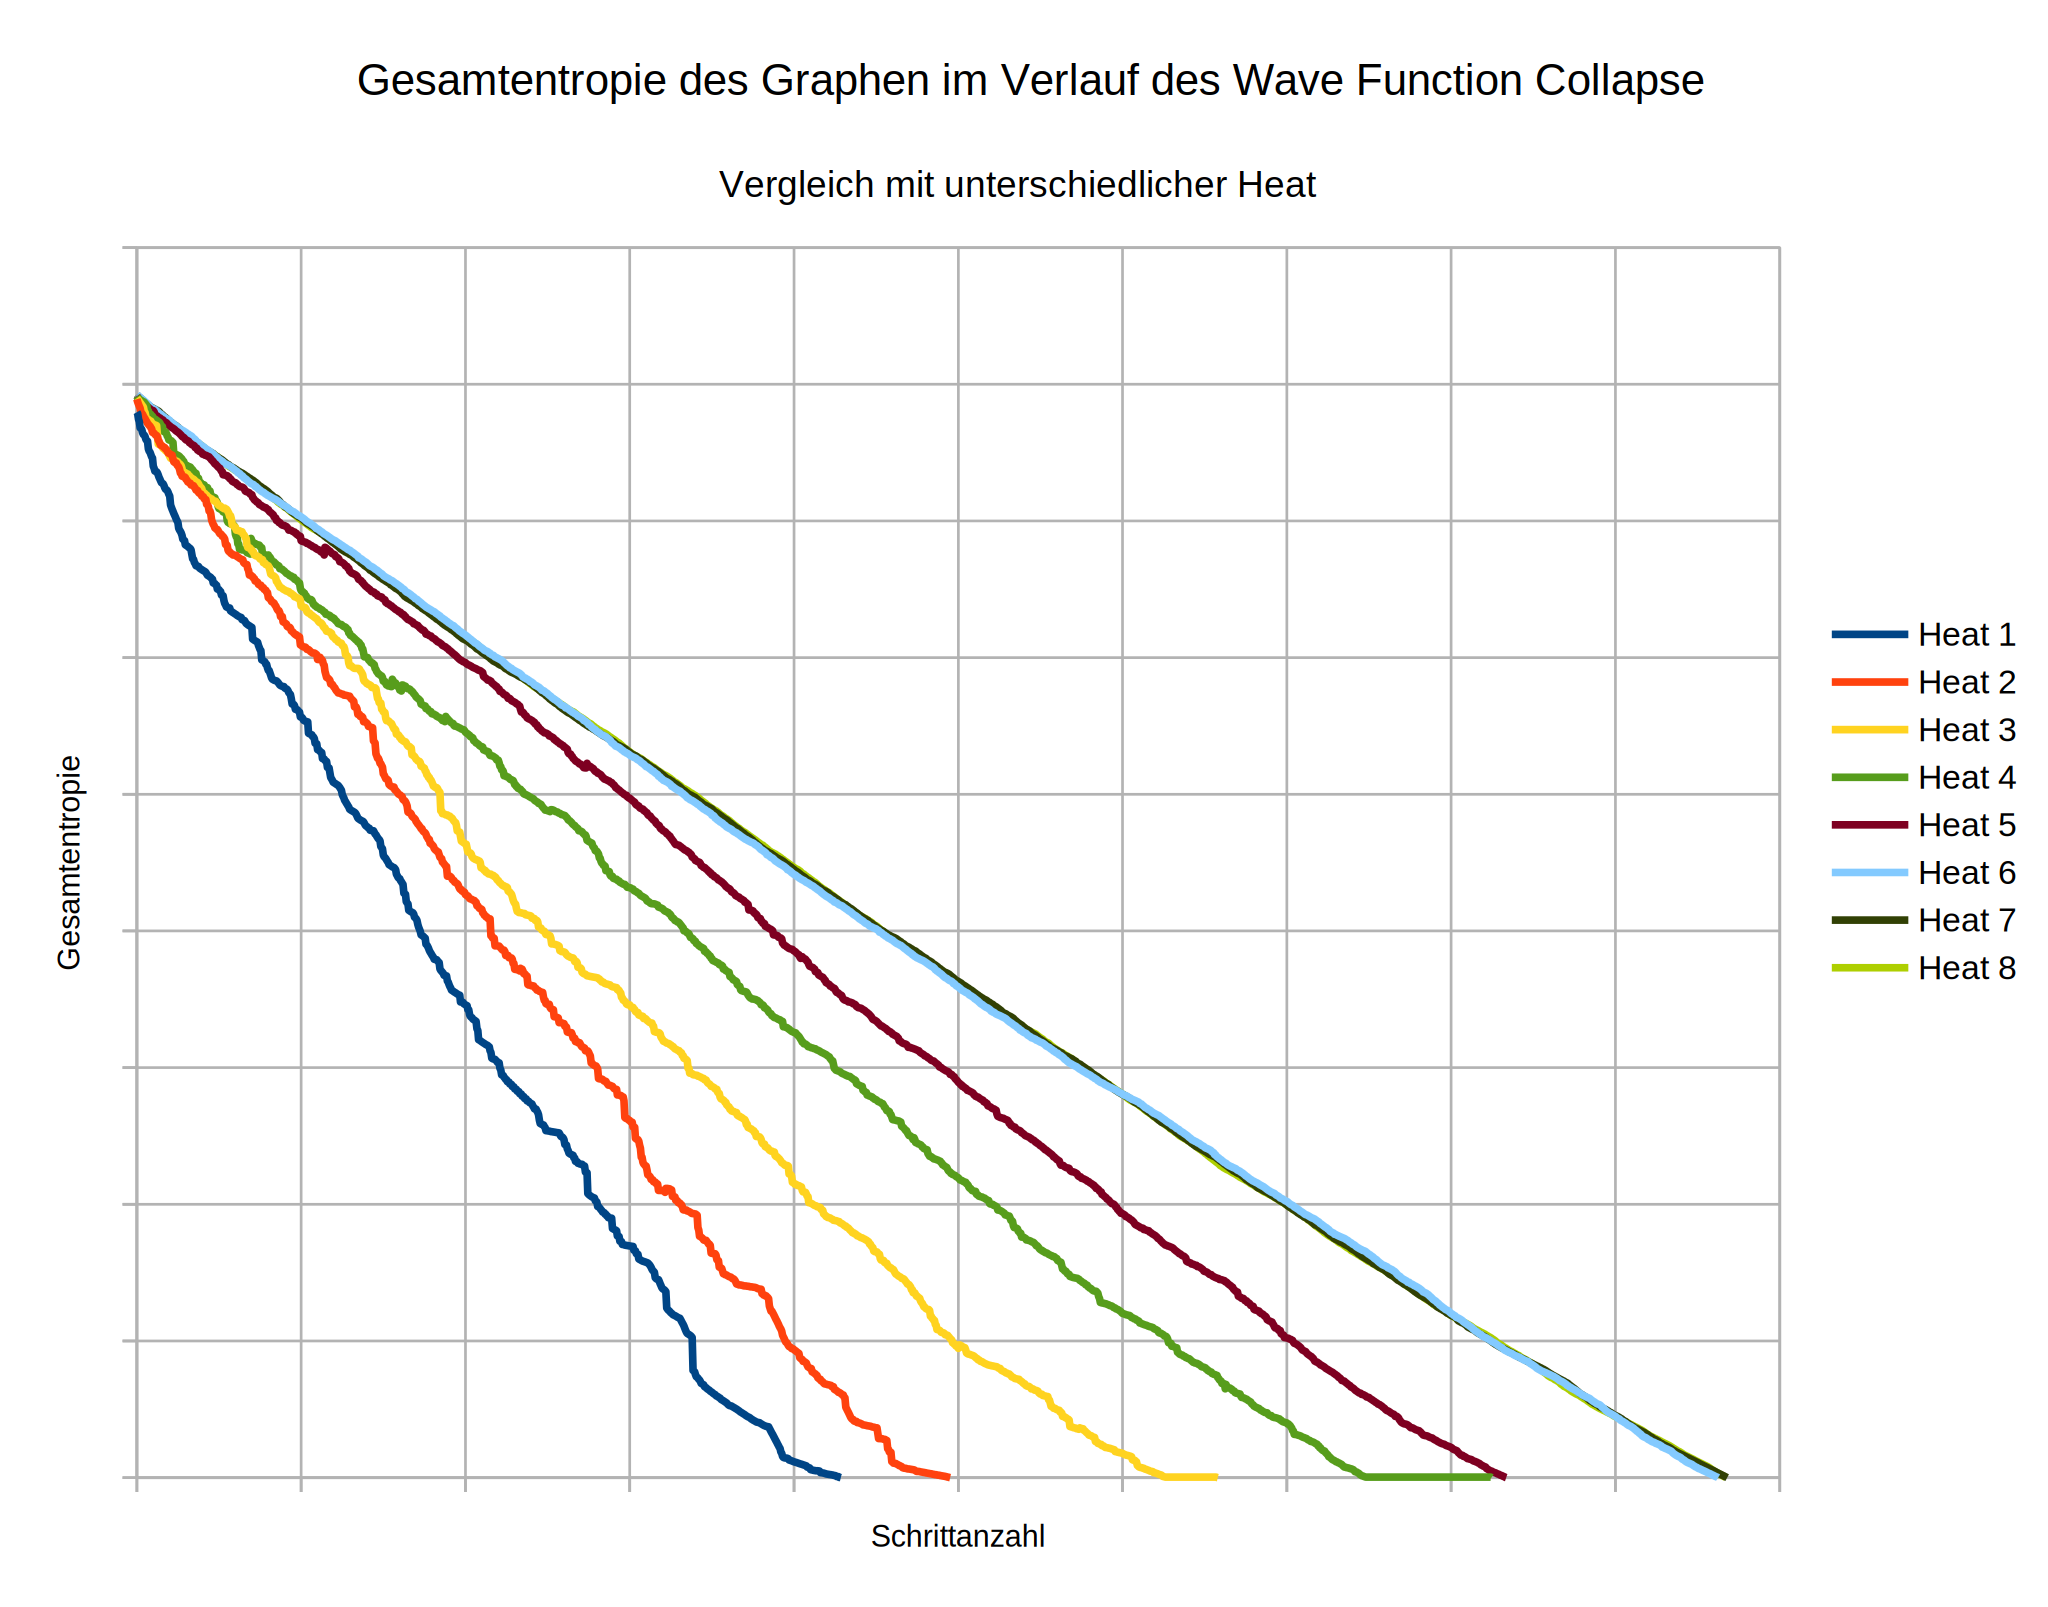
\includegraphics[width=\linewidth]{data/app/1.png}
    
    \caption{
        Screenshot der Anwendung. Oben-Links sind Beispiele zur Auswahl aufgelistet und Wrapping kann eingestellt werden. Mitte-Links kann der Graph generiert werden. Unten-Links kann Heat eingestellt werden und der Wave Function Collapse kann gestartet/neugestartet werden. Man kann auch zu vorherigen Schritten zurückspulen um diese genauer zu betrachten. Auf der rechten Seite sind Menüs mit ein paar Informationen und Einstellungen um andere Daten anzuzeigen oder auszublenden.
    }
    \label{fig:app}
\end{figure}